\section{What is \Md?}
\label{sec:background}

\begin{figure}[t]
\centering
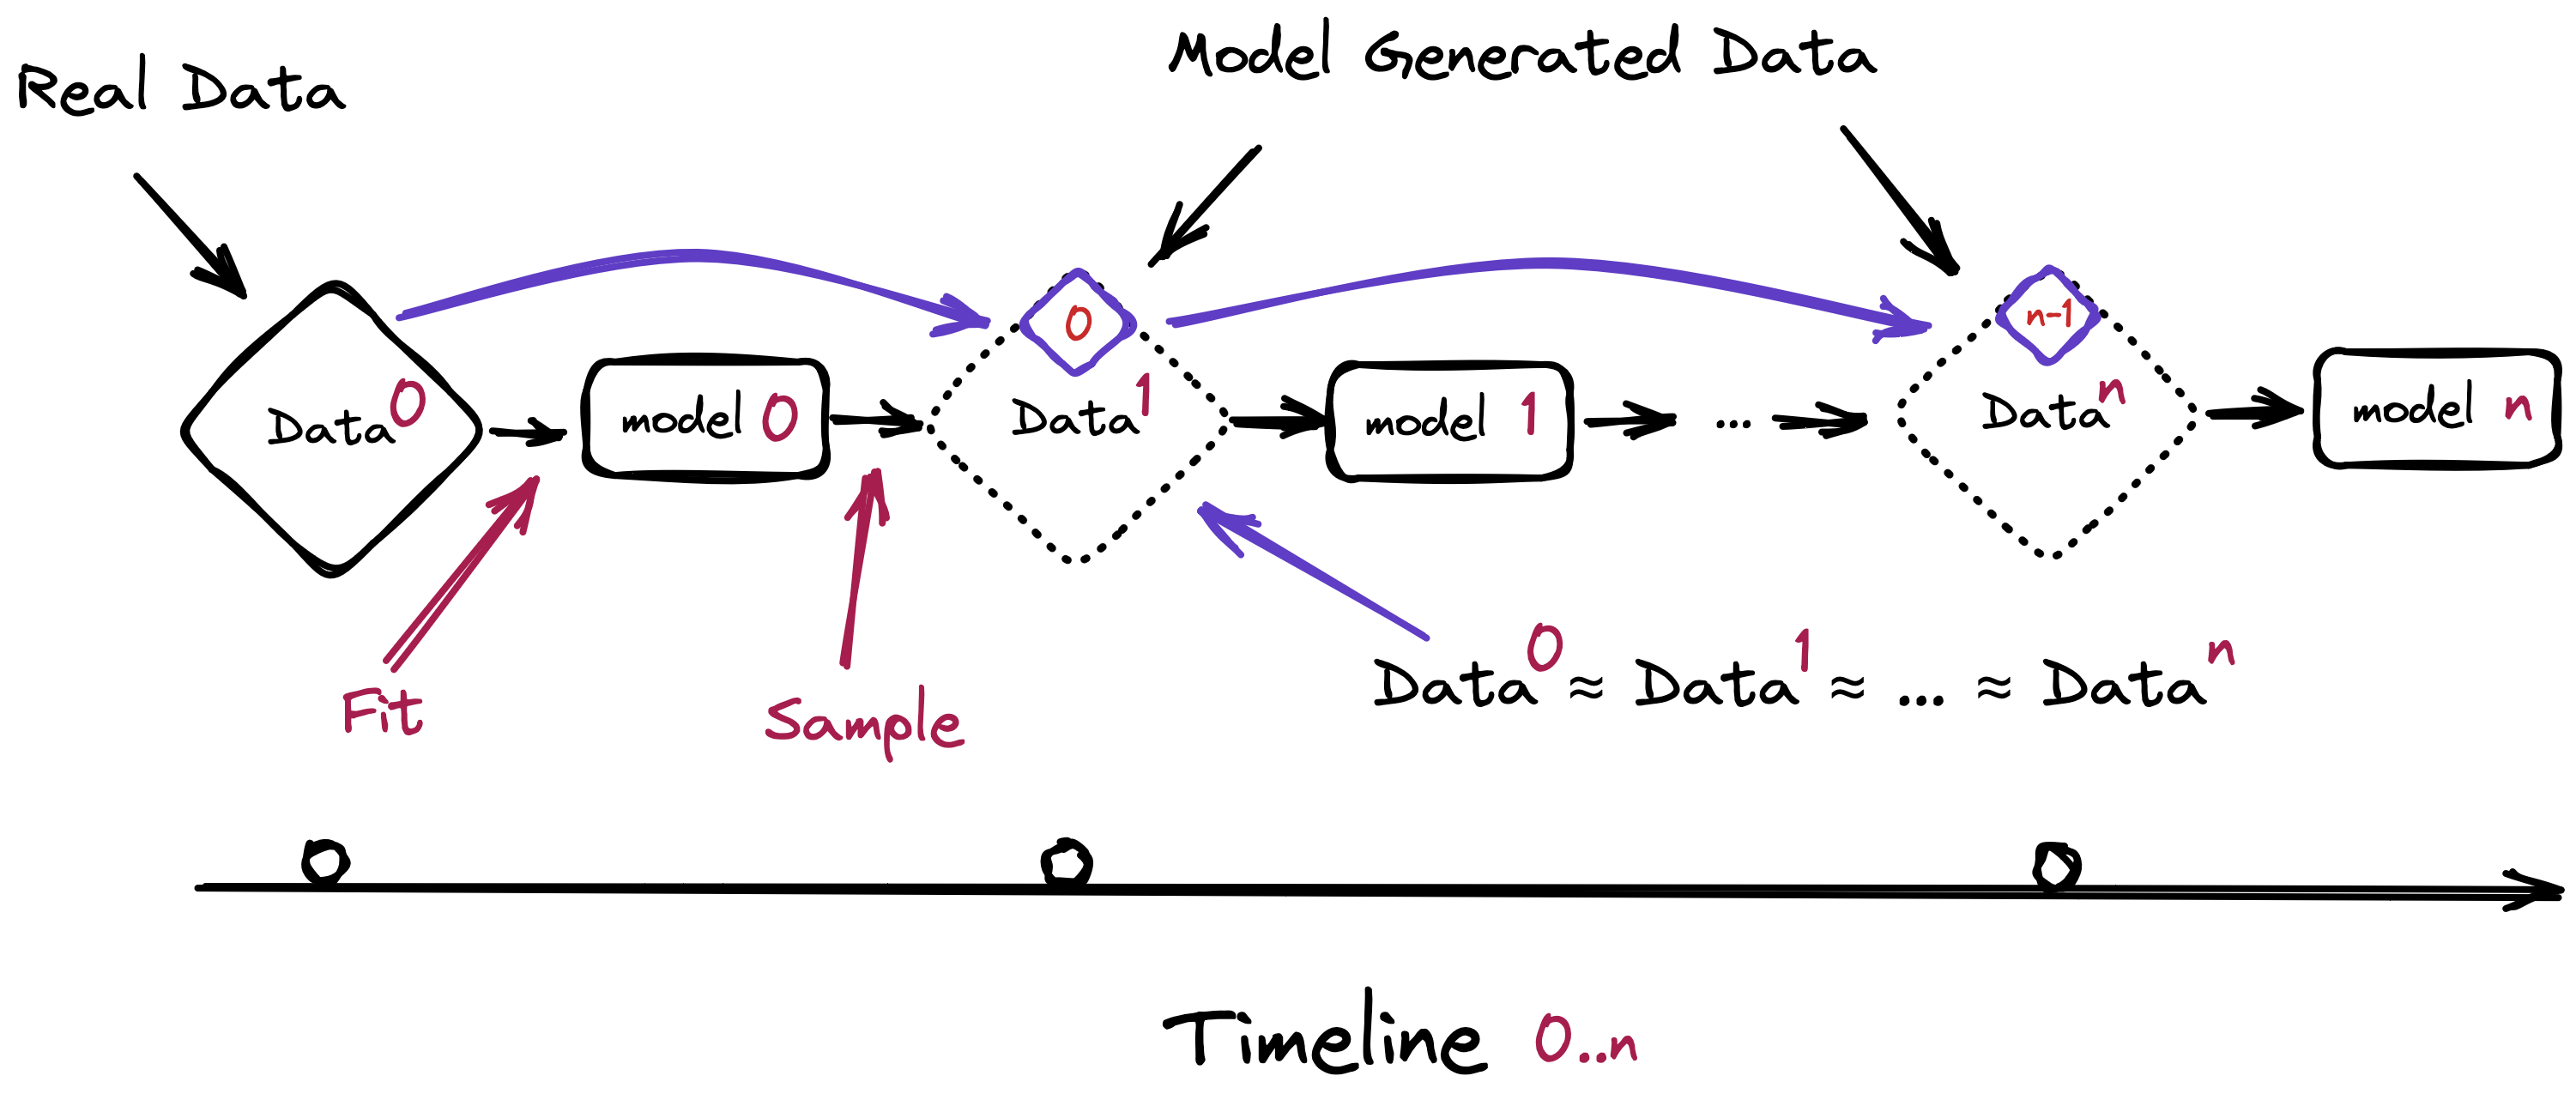
\includegraphics[width=.8\linewidth]{images/infographics/timeline.png}
\caption{The high-level description of the feedback mechanism in the learning process. Here, data are assumed to be human-curated and start off clean; then model $0$ is trained and data are sampled from it; at step $n$, data are added to the overall data from step $n-1$, and this ensemble is used to train model $n$.  Data obtained with Monte Carlo sampling should ideally be statistically close to the original, provided \textit{fitting} and \textit{sampling} procedures are perfect. This process depicts what happens in real life with the Internet -- model-generated data become pervasive. }
\label{fig:highlevel_disc}
\end{figure}

\begin{definition}[\Md]
\Md~is a degenerative process affecting generations of learned generative models, where generated data end up polluting the training set of the next generation of models; being trained on polluted data, they then mis-perceive reality. We separate two special cases: \textbf{early~\md} and \textbf{late~\md}. In early~\md~the model begins losing information about the tails of the distribution; in the late~\md~model entangles different modes of the original distributions and converges to a distribution that carries little resemblance to the original one, often with very small variance. 
\end{definition}

Note that this process is different from the process of \textit{catastrophic forgetting} in that we are considering multiple models over time, in which our models do not forget previously learned data, but rather start misinterpreting what they believe to be real, by reinforcing their own beliefs.

This process occurs due to two specific sources of error compounding over generations and causing deviation from the original model. Of these, one source of error plays a primary role, and in the absence of it, the process would not occur beyond the first generation.

\subsection{Causes of \md}
\label{sec:sourceerror}

There are two main causes for \md, one primary and one secondary, which we describe now. Further mathematical intuition is provided in \Cref{sec:theoreticalint} to explain how these give rise to the errors observed, how different sources can compound and how we can quantify the average model divergence rate. 
\begin{itemize}
    \item \textit{Statistical approximation error} -- this is the primary type of error, which arises due to the number of samples being finite, and disappears as the number of samples tends to infinity. This occurs due to a non-zero probability that information can get lost at every step of re-sampling. \Cref{fig:single_dim_gaus_approx} shows an example of an approximation error. Here, a single-dimensional Gaussian is being approximated from a finite number of samples. Despite using a very large number of points, the errors remain significant; with $10^7$ samples we estimate the mean to be $0.00024899 \pm 1.89382984e^{-4}$, when the true value is $0$.
    \item \textit{Functional approximation error} -- this is a secondary type of error, which stems from our function approximators being insufficiently expressive (or sometimes too expressive outside of the original distribution support~\citep{nguyen2015deep}). It is well known that neural networks are universal functional approximators in the limit, but in practice this is not always true. In particular, a neural network can introduce non-zero likelihood outside of the support of the original distribution. A simple example of this error is if we were to try fitting a mixture of two Gaussians with a single Gaussian. Even if we have perfect information about the data distribution, model errors will be inevitable. It is important to also note that in the absence of statistical error, functional approximation error only occurs at the first generation. Once the new distribution belongs to the image of functional approximator, it remains exactly the same over the generations.
\end{itemize}

Each of the above can cause \md~to get worse or better. Better approximation power can even be a double-edged sword -- better expressiveness may counteract statistical noise, resulting in a good approximation of the true distribution, but it can equally compound this noise. More often then not, we get a cascading effect where combined individual inaccuracy causes the overall error to grow. Overfitting the density model will cause the model to extrapolate incorrectly and might give high density to low-density regions not covered in the training set support; these will then be sampled with arbitrary frequency.

It is worth mentioning that modern computers also have a further computational error coming from the way floating point numbers are represented. This error is not evenly spread across different floating point ranges, making it hard to estimate the precise value of a given number. Such errors are smaller in magnitude and are fixable with more precise hardware, making them less influential on~\md.







\section{Theoretical intuition}
\label{sec:theoreticalint}

In this section we aim to provide a theoretical intuition for the phenomenon of \md. We argue that the process of \md~is universal among generative models that recursively train on data generated by previous generations. We construct toy mathematical models, which prove to be simple enough to provide analytical expressions for quantities of interest, but also portray the phenomenon of \md. We aim to quantify how different sources of error can affect the overall end approximation of the original distribution. As discussed in \Cref{sec:sourceerror}, there are two main sources we are interested in -- \textit{statistical} error and \textit{functional} error. Since in the real world one rarely has infinite samples, quantifying the functional approximation error alone is of little interest for discussion of \md. Therefore, we will examine two simple cases: a discrete distribution in the absence of functional approximation error and a single dimensional Gaussian case, which portrays how functional approximation error can compound with statistical error. 

The overall stochastic process we are going to be considering (which we call \textit{Learning with Generational Data}) is the following. Assume that at generation $i$ we have a dataset $\mathcal{D}_i$ comprising of i.i.d. random variables $X^i_j$, where $j \in \{1,\dots,M_i\}$ denotes the sample number at generation $i$ and $M_i\geq2$. We will denote the distribution of $X^i$ as $p_i$. Here we assume that $p_0$ denotes the original distribution, from which the data comes from. Going from generation $i$ to generation $i+1$, we aim to estimate the distribution of samples in $\mathcal{D}_i$, with an approximation $p_{\theta_{i+1}}$. This step is what we refer to as functional approximation $\mathcal{F_\theta}: p_i \to p_{\theta_{i+1}}$. We then resample the dataset $\mathcal{D}_{i+1}$ from the distribution $p_{i+1} = \alpha_i p_{\theta_{i+1}} + \beta_i p_{i} + \gamma_ip_0$, with non-negative parameters $\alpha_i, \beta_i, \gamma_i$ summing up to $1$, \ie~they represent proportions of data used from different generations. This corresponds to a mixing of data coming from the original distribution ($\gamma_i$), data used by the previous generation ($\beta_i$) and data generated by the new model ($\alpha_i$). We refer to this as the sampling step. For the mathematical models to come, we consider $\alpha_i=\gamma_i=0$ \ie~data only from a single step is used, while numerical experiments are performed on more realistic choices of parameters. 

\subsection{Discrete distributions with exact approximation}
In this subsection we consider a discrete probability distribution, which is represented by a histogram, \eg~as shown on \Cref{fig:histograms}. In what follows we consider the stochastic process in absence of functional approximation error, \ie~\;$\mathcal{F}(p)=p$. In this case, \md~arises only due to statistical errors from the sampling step. At first, the tails (low probability events) begin to disappear due to low probability of sampling them, and over time the distribution becomes a delta function. Denoting the sample size as $M$, if we consider state $i$ with probability $q\leq\frac{1}{M}$, the expected number of samples with value $i$ coming from those events will be less than $1$, which means that in practice we will lose information about them. This is portrayed on \Cref{fig:histograms}, where infrequent events get cut off. Considering more generally some state $i$ with probability $q$, using standard conditional probability one can show that the probability of losing information (\ie~sampling no data at some generation) is equal to $1-q$. But this in turn means that we must converge to a delta function positioned at some state, and the probability of ending up at a certain state is equal to the probability of sampling said state from the original distribution.

But how do we show directly that this process is going to turn our distribution into a delta function? By considering the process as going from $\mathbf{X}^i\to\mathcal{F_\theta}\to p_{i+1}\to\mathbf{X}^{i+1}$, we see that this forms a Markov Chain, as $\mathbf{X}^{i+1}$ only depends on $\mathbf{X}^{i}$. Furthermore, if all the $X^{i}_j$ have the same value, then at the next generation the approximated distribution will be exactly a delta function, and therefore all of $X^{i+1}_j$ will also have the same value. 
\begin{figure}
    \centering
    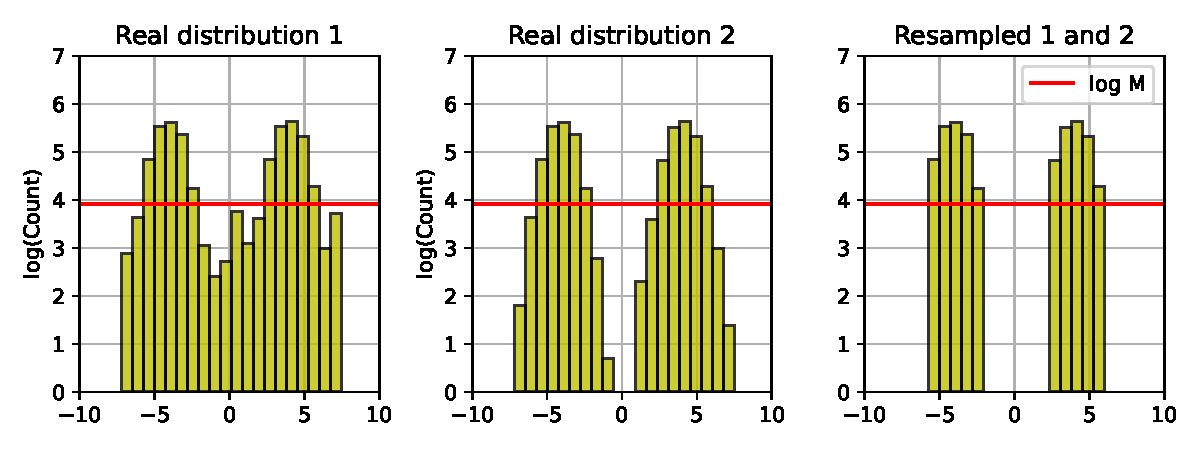
\includegraphics[width=0.9\linewidth]{images/singlegaus/hist_ex.pdf}
    \caption{Shown in the middle is a histogram plot of samples from a Gaussian mixture with means $(-4,4)$ and variances of $1$. To the left of it is a similar distribution, but with 'fatter' tails, and on the right the same histograms are shown, but with low probability events being cut off due to finite resampling. Although distributions 1 and 2 are very different, when resampled (only assuming the expected behaviour), the tails get cut off, leading to the same observed distribution. In this case this is all states with probability less than $1/M$, or equivalently, bins with $\log{\texttt{Count}}\leq\log{M}$.}
    \label{fig:histograms}
\end{figure}
This implies that the Markov chain contains at least one absorbing state, and therefore with probability 1 it will converge to one of the absorbing states. This is a well-known fact, of which a proof is provided in \Cref{ap:markov}. For this chain, the only absorbing states are those corresponding to delta functions. As a result, as we follow the progress of \md, we are guaranteed  to end up in a constant state, having lost all the information of the original distribution when the chain is absorbed.\footnote{This argument also works in general due to floating point representations being discrete, making the Markov Chain over the parameters of the model discrete. Thus as long as the model parameterisation allows for delta functions, we \textit{will} get to it, as due to sampling errors the only possible absorbing states are delta functions.} Based on the discussion above we see how both early and late stage \md~ must arise in the case of discrete distributions with perfect functional approximation.






\begin{figure}%
    \centering
    \subfloat[\centering Mean estimation]{{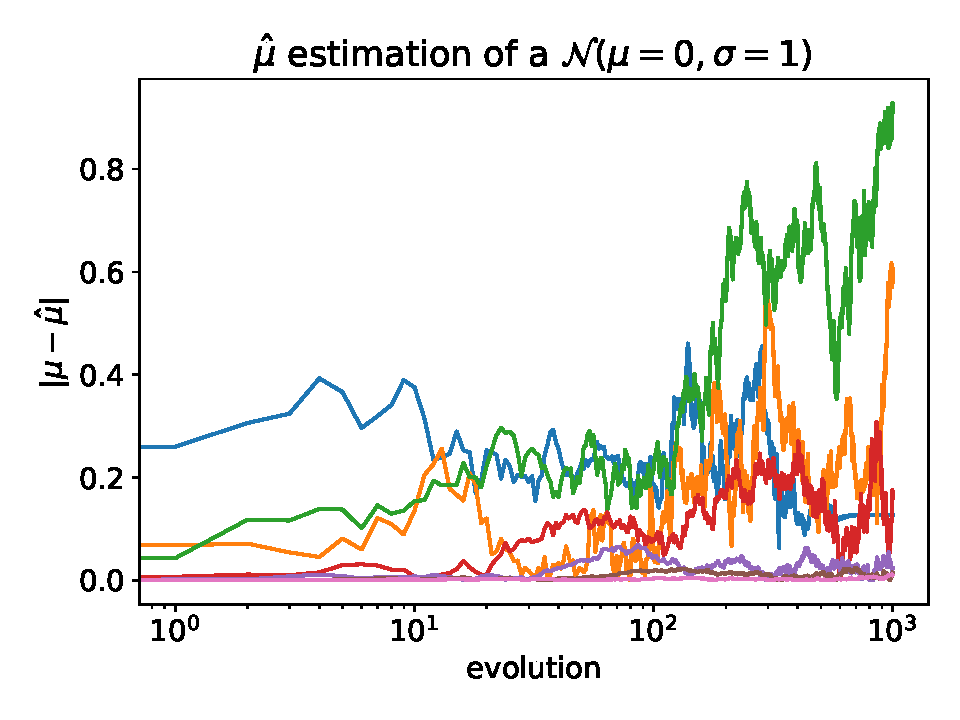
\includegraphics[width=0.43\textwidth]{images/singlegaus/single_normal_approx_mu.pdf} }}%
    \subfloat[\centering Standard Deviation]{{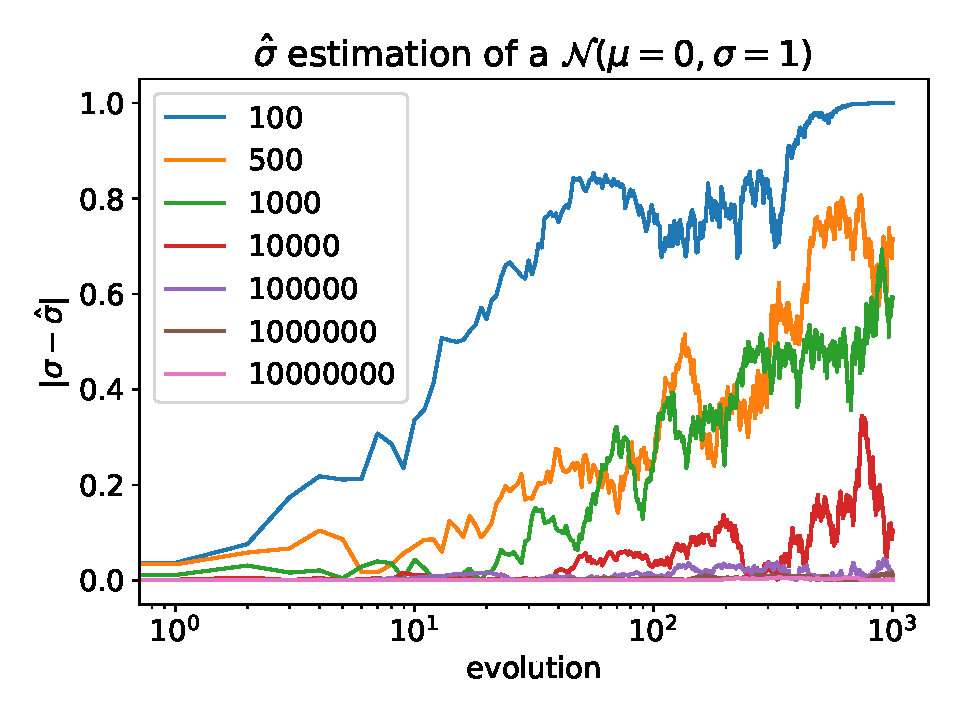
\includegraphics[width=0.43\textwidth]{images/singlegaus/single_normal_approx_sigma.pdf} }}%
    \caption{Recursive fitting-sampling of a 1D Gaussian with different numbers of samples drawn. We find that unless sampled a very large number of times,~\ie~<100000, both standard deviation and mean get significantly affected. Here we report a single run; while re-running the experiment changes the initial performance, both $\mu$ and $\sigma$ drift over time. The overall graph looks quite similar to that of a Gaussian random walk.}%
    \label{fig:example1}%

    \centering
    \subfloat[\centering Mean estimation]{{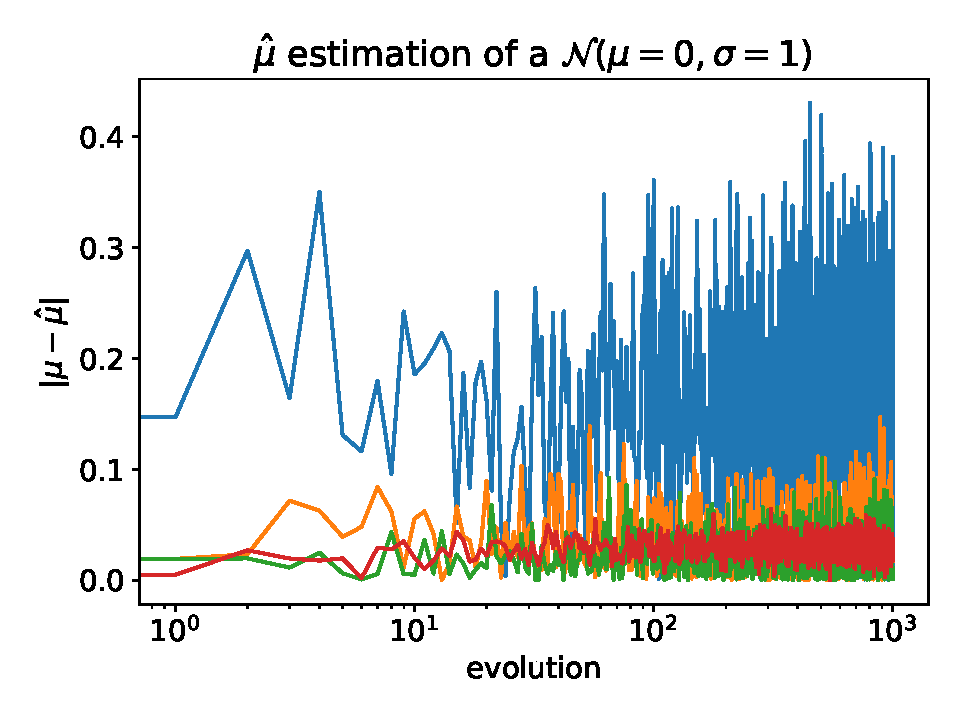
\includegraphics[width=0.43\textwidth]{images/singlegaus/alldat_samp_single_normal_approx_mu.pdf} }}%
    \subfloat[\centering Standard Deviation]{{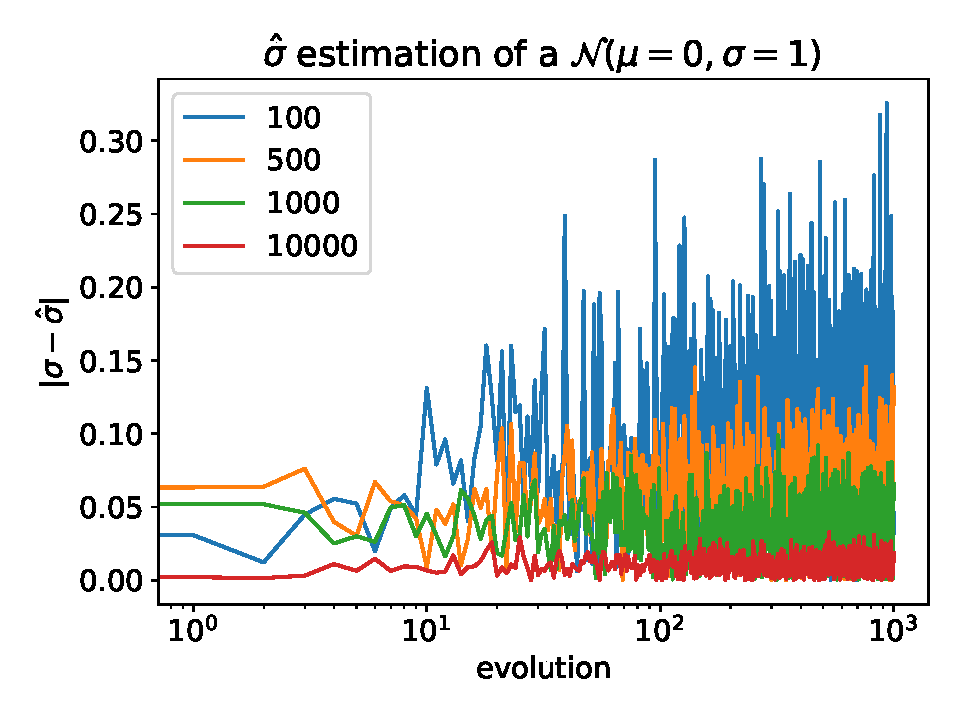
\includegraphics[width=0.43\textwidth]{images/singlegaus/alldat_samp_single_normal_approx_sigma.pdf} }}%
    \caption{Recursive fitting-sampling of a 1D Gaussian with different numbers of samples drawn. In this plot data get accumulated in a pool, from which a fixed sample is drawn. In other words, a model $n$ gets data sampled, its output is mixed with data sampled from models $1\dots n$, and then the mix gets sampled to fit the model $n+1$. The uncertainty arising from all of the different modalities appearing in data causes the distribution parameters to jump around quite significantly.}%
    \label{fig:example2}%

    \centering
    \subfloat[\centering Mean estimation]{{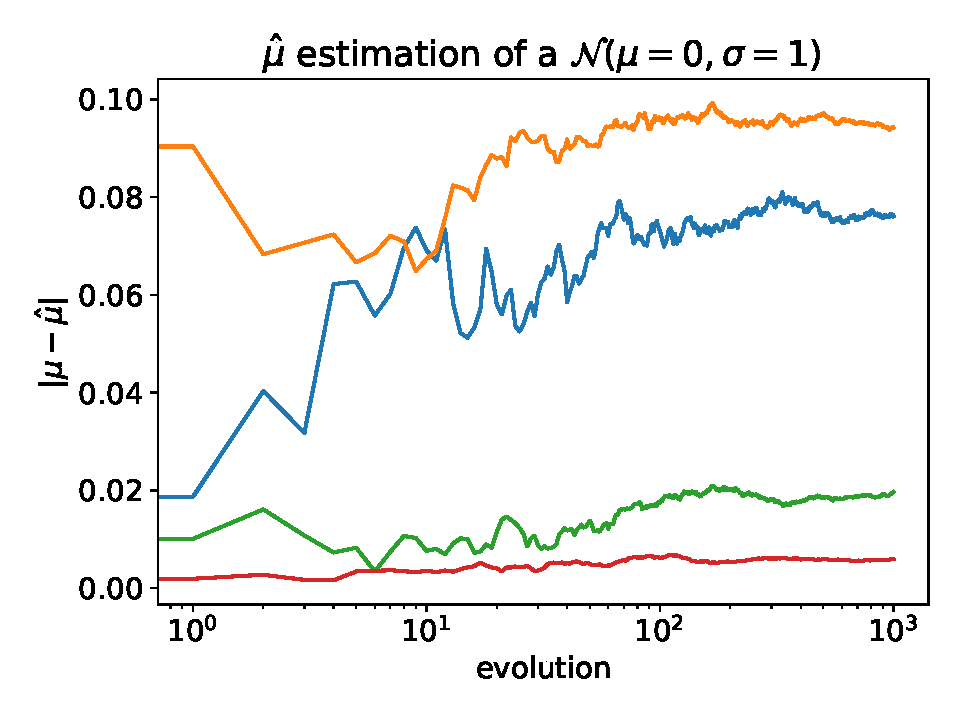
\includegraphics[width=0.43\textwidth]{images/singlegaus/alldat_single_normal_approx_mu.pdf} }}%
    \subfloat[\centering Standard Deviation]{{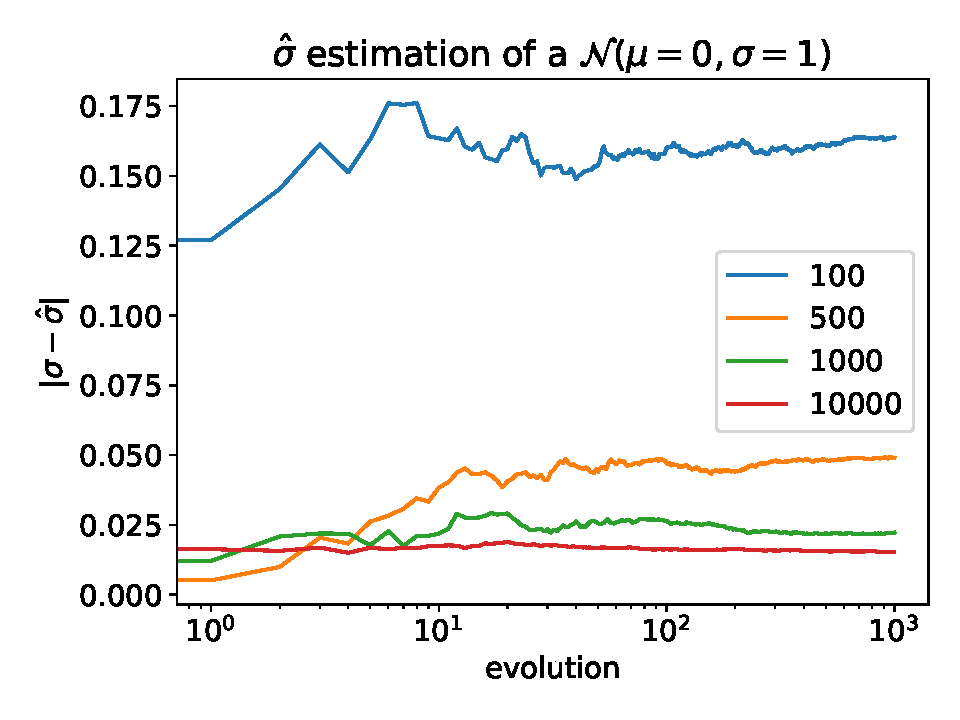
\includegraphics[width=0.43\textwidth]{images/singlegaus/alldat_single_normal_approx_sigma.pdf} }}%
    \caption{Recursive fitting-sampling of a 1D Gaussian with different number of samples drawn. In this plot data are accumulated in a pool, all of which is used to fit a model. In other words, a model $n$ gets data sampled, its output mixed with data sampled from models $1\dots n$, and then the result is used to fit the model $n+1$. Over time the variance in estimates reduces due to linear growth of data.}%
    \label{fig:example3}%
\end{figure}


\subsection{Single dimensional Gaussian}

Following the discussion about discrete distributions, we now move on to considering how both functional approximation error and sampling error can compound (or cancel out) the process of~\md. 

To demonstrate this, consider a single dimensional Gaussian $X^0 \sim \mathcal{N}(\mu,\sigma^2)$. If we have full faith in the data we observe, the functional approximation involves estimating sample mean and variance and fitting a single dimensional Gaussian. We can estimate them using the unbiased sample mean and variance estimators:
\begin{align}
\label{eq:estimates_gaussian}
    \mu_{i+1} &= \frac{1}{M_i}\sum_j X^i_j; \quad \sigma_{i+1}^2 = \frac{1}{M_i-1}\sum _j(X^i_j-\mu_{i+1})^2.
\end{align}


Note here, that if we were to use maximum likelihood estimation, we would instead arrive at a biased variance estimator. With these estimates, the functional approximation step simply corresponds to considering a normal distribution with these parameters, which we can sample from: 
\begin{equation}
X^{i+1}_j|\mu_{i+1},\;\sigma_{i+1}\sim \mathcal{N}(\mu_{i+1},\sigma_{i+1}^2).
\end{equation}
This provides us with the conditional distribution of $X^i_j$, which allows us to calculate the full distribution of $X^i_j$. From \Cref{eq:stochproc}, we see that even after the first approximation, the distribution of $X^i_j$ is no longer normal, it follows a variance-gamma distribution \citep{fischer2023variancegamma}. However, instead of writing the probability density function at each generation, we can explicitly construct them in terms of independent random variables. In particular, it is well known \citep{cochran_1934} that $\mu_1$ and $\sigma_1$ are independent, with $\mu_1 \sim \mathcal{N}(\mu, \frac{\sigma^2}{M_0})$ and $(M_0-1)\sigma_1^2 \sim \sigma^2\Gamma(\frac{M_0-1}{2}, \frac12)$. In what follows we will denote with $Z$ random variables that are distributed with $\mathcal{N}(0, 1)$ and with $S^i$ random variables that are distributed with $\frac{1}{M_{i-1}-1}\Gamma(\frac{M_{i-1}-1}{2}, \frac12)$. 

\begin{align}
\label{eq:stochproc}
    X^0_j &= \mu + \sigma Z^0_j; \quad X^1_j = \mu + \frac{\sigma}{\sqrt{M_0}}Z^1 + \sigma\sqrt{S^1}Z^1_j; \quad \dots\\
    \nonumber X^n_j &= \mu + \frac{\sigma}{\sqrt{M_0}}Z^1 + \frac{\sigma}{\sqrt{M_1}}\sqrt{S^1}Z^2 + \dots + \frac{\sigma}{\sqrt{M_{n-1}}}\sqrt{S^1\times\dots\times S^{n-1}}Z^n+\sigma\sqrt{S^1\times\dots\times S^{n}}Z^n_j.
\end{align}

These are not joint distributions, as $Z^n$ and $S^n$ depend directly on $Z^{n-1}_j$, but when considering $X^n_j$ on its own the formula above provides all the information about the full distribution. %

The first thing we may try calculating is the variance. It is possible to find its exact value, but the mean and variance of the square root of gamma distribution are expressed in terms of gamma functions, making the result quite clunky. In what follows, we will expand everything to second order in each of $(1/M_i)$ as we assume each sample size to be large (in practice this becomes quite accurate after $M\sim100$). We then find that 
$$
\frac{1}{\sigma^2}\operatorname{Var}(X^n_j) = \frac{1}{M_0}+\frac{1}{M_1}+ \dots + \frac{1}{M_{n-1}}+1 + \mathcal{O}(2).
$$

And if we were to assume that $M_i = M$ are constant, we would find that:
$$
\operatorname{Var}(X^n_j) = \sigma^2\left(1+\frac{n}{M}\right); \quad \mathbb{E}(X^n_j) = \mu.
$$
This means that as $n\to\infty$, the variance diverges linearly. This is the same scaling as for a single dimensional Gaussian random walk. We can further see the similarities in numerical experiments shown on \Cref{fig:example1} for a range of different sample sizes, confirming these theoretical intuitions.

Even though the variance of $X^n_j$ diverges, it does not provide us with any information of what the corresponding estimates of $\mu_{n+1}$ and $\sigma^2_{n+1}$ are, or how far they are from the original $\mu$ and $\sigma$. In particular, we may want to consider what the distance would be between the true distribution and the approximated distribution at step $n+1$. To measure this we can consider the Wasserstein-2 distance between two normals:
\begin{equation*}
R^{n+1}_{W_2} := W^2_2\left(\mathcal{N}(\mu,\sigma^2),\mathcal{N}(\mu_{n+1},\sigma^2_{n+1})\right)=\|\mu_{n+1}-\mu\|^2 + \|\sigma_{n+1}-\sigma\|^2
\end{equation*}
Now we can calculate the risk that occurs due to finite sampling, \ie~what the expected value of the distance is (expanding in $1/M_i$): 
\begin{align}
\label{eq:mean_risk}
\mathbb{E}_{\mu_{n+1},\sigma_{n+1}^2}\left[R^{n+1}_{W_2}\right]&=\frac{3}{2}\sigma^2\left(\frac{1}{M_0}+\frac{1}{M_1}+ \dots + \frac{1}{M_{n}}\right)+\mathcal{O}(2),\\
\operatorname{Var}_{\mu_{n+1},\sigma_{n+1}^2}\left[R^{n+1}_{W_2}\right]&=\frac{1}{2}\sigma^4\left(\frac{3}{M_0^2}+\frac{3}{M_1^2}+ \dots + \frac{3}{M_{n}^2} + \sum_{i\neq j}\frac{4}{M_iM_j}\right)+\mathcal{O}(3).
\end{align}

This result allows us to interpret exactly what occurs in this formulation of \md. To be precise, due to errors occurring from re-sampling the approximated distribution, each generation ends up corresponding to a new step in a random walk of model parameters. The risk that occurs in this model ends up diverging for a constant sample size at each generation. In order for the end distribution approximation to be accurate, and for the distance to be finite, the sampling rate $M_i$ needs to increase superlinearly, \ie~one needs to collect increasingly more samples over time, perhaps quadratically. However, even in that case the expected distance after $n$ steps remains non-zero and the only case in which it does in fact end up being $0$ is when sampling is infinite at each step. Overall, this only shows us how far on average we go from the original distribution, but the process can only 'terminate' if the estimated variance at a certain generation becomes small enough, \ie~we effectively turn into a delta function. 

Shown on \Cref{fig:example2,fig:example3} are different runs of this process for different values of parameters of $\alpha_i, \beta_i, \gamma_i$ for different sample sizes, which was investigated numerically to see whether they can be enough to overcome \md, however even in those cases the changes are inevitable, although attenuated.


\subsection{Noisy approximation model}
\label{sec:noisyapprox}
With the simple example out of the way, we can now construct a lower bound on the distance of generation $n$ distribution from the original and show that without superlinear sampling it similarly diverges in the limit of large $n$.
A nice property of Wasserstein-2 distance is that Gaussians provide a universal lower bound for the Wasserstein distance \citep{gelbrich1990formula}. In particular, for $\kappa$ and $\nu$  probability measures on a Euclidean $N$-dimensional space with $\mu_\kappa$ and $\mu_\nu$ means, $\Sigma_\kappa$ and $\Sigma_\nu$ covariance matrices, we have that
$$
W^2_2(\kappa, \nu) \geq\left\|\mu_\kappa-\mu_\nu\right\|^2+
\operatorname{Tr}\left(\Sigma_\kappa+\Sigma_v-2\left(\Sigma_\kappa^{1 / 2} \Sigma_v \Sigma_\kappa^{1 / 2}\right)^{1 / 2}\right)\geq\left\|\mu_\kappa-\mu_\nu\right\|^2
$$
With this, instead of quantifying the distance exactly, we can instead lower bound it. The only limitation is that we are going to have to specify a functional approximation model. In order to achieve a $W_2$ bound, we will be required to specify how the mean changes between generations. In the scenario where we only have access to the sample mean, we would approximate the mean of the next generation distribution as \Cref{eq:estimates_gaussian}. However, as more information arrives, or the model begins using it better, we may end up diverging from the sample mean. We would still require that the model have good performance, \ie~on average the mean estimate is the same. We will also have to specify expected behaviour of the model over the the variance calculation, which once again will be chosen such that it averages out. Thus, we will adopt the following evolution over generations:
\begin{equation}
    \mu_{i+1}=\frac{1}{M_i}\sum_jX^i_j+\varepsilon_{i+1}=\frac{\Sigma^{1/2}_i}{\sqrt{M_i}}T^{i+1}+\mu_i+\varepsilon_{i+1}; \quad\mathbb{E}_{X^i_j}(\Sigma_{i+1})=\Sigma_i
\end{equation}
where we define $T^{i+1}$ to satisfy the equation above,~\ie~ $T^{i+1}=\frac{\Sigma^{-1/2}_i}{\sqrt{M_i}}\sum_j\left(X^i_j-\mu_i\right)$. With this normalisation $T$ has mean $0$ and covariance $I_N$ and by the central limit theorem (CLT) we would have $T^{i+1}|\mu_i,\Sigma_i\overset{\mathcal{D}}{\to}\mathcal{N}(0,I_N)$, however the lower bound will not rely on this.  
To arrive at a lower bound for the risk, similar to that of \Cref{eq:mean_risk}, we are going to have to make a few assumptions about the form of $\varepsilon_{i+1}$.\\
\textbf{Assumptions}:
\begin{enumerate}
    \item On average we can capture the mean to be the same as at the iteration prior: 
    \begin{equation}
        \mathbb{E}[\varepsilon_{i+1}|\mu_i,\Sigma_i]=0
    \end{equation}
    \item Given all of $X^i_j$, epsilon must be constant, \ie~it is a function of only the data:
    \begin{equation}
        \varepsilon_{i+1} = \varepsilon_{i+1}\left(X^i_j\right)
    \end{equation}
    In particular, it is dependent on $\mu_i$ and $\Sigma_i$ only through the data.
    \item The extra noise is orthogonal to the sample mean in the sense of random variables. This is effectively assuming that the noise does not contain any first moment information, \ie~we have:
    \begin{equation}
        \operatorname{Cov}(\varepsilon_{i+1},T^{i+1}|\mu_i,\Sigma_i)=0
    \end{equation}
    This may seem like a rather strong assumption, compared to the previous ones, however this property can be shown to hold true when imposing CLT on $T^{i+1}$ in the limit of large $M_i$ (note here that $M_i$ can only be assumed to be \textbf{large}, and not infinite) and assuming that $\varepsilon$ is strictly a function of moments higher than first. \\
    Furthermore, a property of this type is necessary to actually provide any information, since prior to it there would be no need to separate into an epsilon term and a sample mean term, since all could be absorbed into $\varepsilon$. 
\end{enumerate}
In \Cref{ap:alternative}, we further provide an alternative to Assumption 3, wherein by bounding the size of noise we are able to recover a similar bound, but only as an expansion in $1/M_i$.
\\
With all the assumptions in place, we now have the following bound:
\begin{align}
\label{eq:mean_risk_2}
\mathbb{E}\left[R^{i+1}_{W_2}\right]&\geq\mathbb{E}\left(\|\mu_{i+1}-\mu\|^2\right)\\&=\mathbb{E}\left(\|\mu_{i}-\mu\|^2\right)+\mathbb{E}\left(\|\varepsilon_{i+1}\|^2\right)+\frac{1}{M_i}\mathbb{E}\left((T^{i+1})^{\top}\Sigma_i(T^{i+1})\right)+\\&+\frac{2}{\sqrt{M_i}}\mathbb{E}\left((\varepsilon_{i+1})^{\top}\Sigma^{1/2}_iT^{i+1} + (\mu_i-\mu)^{\top}\Sigma^{1/2}_iT^{i+1} \right)\\&=\mathbb{E}\left(\|\mu_{i}-\mu\|^2\right)+\frac{\operatorname{Tr}\Sigma}{M_i}+\mathbb{E}\left(\|\varepsilon_{i+1}\|^2\right)+\frac{2}{\sqrt{M_i}}\mathbb{E}\left((\varepsilon_{i+1})^{\top}\Sigma^{1/2}_iT^{i+1} \right)
\end{align}
Now the only quantity to evaluate is 
\begin{equation}
    \frac{2}{\sqrt{M_i}}\mathbb{E}\left((\varepsilon_{i+1})^{\top}\Sigma^{1/2}_iT^{i+1}\right) 
    = \frac{2}{\sqrt{M_i}}\int d\Sigma_i\;p(\Sigma_i)\operatorname{Tr}\left[\Sigma^{1/2}_i\operatorname{Cov}(\varepsilon_{i+1},T^{i+1}|\Sigma_i)\right]=0,
\end{equation}
by Assumption 3. Therefore, the overall bound would be similar to the Gaussian case, but with extra noise variance terms:
\begin{align}
\label{eq:mean_risk_3}
\mathbb{E}_{\mu_{n+1},\sigma_{n+1}^2}\left[R^{n+1}_{W_2}\right]\geq\operatorname{Tr}\Sigma\left(\frac{1}{M_0}+\frac{1}{M_1}+ \dots + \frac{1}{M_{n}}\right)+\sum^{n+1}_{i=1} \mathbb{E}\left(\|\varepsilon_i\|^2\right)
\end{align}

As a result, we have shown that the same superlinear scaling would be required to minimise the lower bound on \md~even in the case of more generic models of approximation, in which the mean at step $i+1$ can be separated orthogonally into the sample mean and 'extra'. 

Overall, the message of this section can be summarised as follows: \\
\fbox{\begin{minipage}{\linewidth}
\emph{When learning on generational data, due to finite sampling, we are only able to \textbf{approximate} the original distribution. While on average we should recover the original distribution, the variance arising from this is non-zero. As a result, over the generations, the average distance of $n$'th generation from the original grows and can become infinite in the limit since errors compound over time.}
\end{minipage}}
